\documentclass{article}
\usepackage[pdftex]{graphicx}
\usepackage{amsmath}
\usepackage{verbatim}
\usepackage{enumerate}
\author{Michael Anderson}
\title{Homework 1}
\begin{document}
\maketitle
\center{CS534}
\center{Prof. Fern}\\
\flushleft
\newpage

\section{Perceptron}

\begin{enumerate}
\item
Did not bother to do this part, because only one training epoch was required
for this batch algorithm to linearly separate the data.

\item
Below are the points in twogaussian.csv together with their correct
classifications, and a linear decision boundary. w = (1.5, -0.629, -0.521)


\includegraphics{perceptron.png}

\end{enumerate}

\newpage

\section{Voted Perceptron}
\begin{enumerate}

\item
From the graph below, it appears that the number of misclassifications of the
iris set
bottomed out at around epoch 10 for this particular run, and in the next 90
epoches the algorithm flailed around slightly,
finally settling at a respectable 5 misclassifications out of 150.

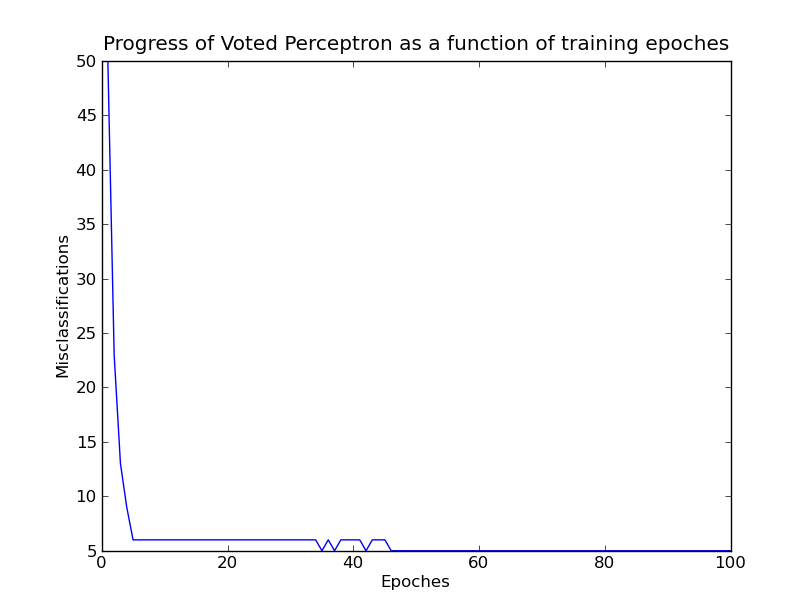
\includegraphics{voted_perceptron_error.png}

\item
Below is a visualization of the calculated voted perceptron boundary for a
sample run on the iris set, using 1000 random points. The linear decision
boundary is clear.


\includegraphics{voted_perceptron.png}

\newpage

\item
Below is the linear decision boundary and plotted points for the voted
perceptron algorithm using $w_i{avg}$. Only half a dozen out of 150 points are
misclassified. w = (1162932, -79670, -481308)

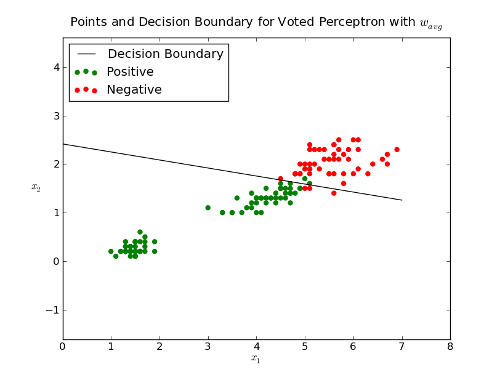
\includegraphics{voted_perceptron_avg.png}

By looking at this graph and the one before it, it is obvious that the
two decision boundaries similar, but not identical. This is because the data
is shuffled randomly between training epoches, which results in slightly
different decision boundaries for each run of the algorithm. Additionally,
using $w_{avg}$ keeps some information that is lost when performing the
$sgn\{wx\}$ calculation in standard voted perceptron, altering the results
slightly.


\end{enumerate}

\end{document}
